\documentclass{beamer}
\title[Android Dev~101] {Intro to App Development on Android}
\subtitle{@~\href{https://thacks.ca}{T.Hacks 2016}}
\author{Marc~Lijour}
\date{Workshop - October 22, 2016}
\subject{Programming Skills}
\usepackage{tikz}
%
\logo{
\includegraphics[scale=.1]{./images/logo-sfl-250.png}}
\AtBeginSection[]
{
  \begin{frame}
    \frametitle{Table of Contents}
    \tableofcontents[currentsection]
  \end{frame}
}
\usetheme{Boadilla}
%\usepackage[format=plain,justification=raggedright,singlelinecheck=false]{caption}
\usepackage[format=plain,justification=justified,singlelinecheck=false]{caption}
\usepackage[utf8]{inputenc}
\usepackage{dirtytalk}
\usepackage{wrapfig}
\usepackage{hyperref}
\usepackage{verbatim}
\usepackage{mathabx}
%\usepackage{MnSymbol}

\begin{document}
\frame{
%	\tikz[remember picture,overlay]
%	  \node at
%		([xshift=2cm,yshift=2cm]current page.south west)
%		%([xshift=10.5cm,yshift=-3cm]current page.west)
%		{
\includegraphics[width=3cm,height=3cm]{./images/logo-sfl-250.png}};
	\titlepage
}

\begin{frame}
\frametitle{Table of Contents}
\tableofcontents[currentsection]
\end{frame}

%%%%%%%%%%%%%% 1st SECTION: Intro %%%%%%%%%%%%%%%%%
\section[Section]{Introductions}
	\begin{frame}
	\frametitle{Presenter: Marc Lijour}
	\framesubtitle{Helping businesses and countries digitize}
	\tikz[remember picture,overlay]
	  \node at
		([xshift=-2.1cm,yshift=-1.5cm]current page.north east)
		{
\includegraphics[width=3cm,height=3cm]{./images/logo-sfl-250.png}};
	%Content goes here
	%\emph{Helping businesses and countries digitize}
	%\vspace{1.2cm}
		\begin{itemize}
			\item Director @ Savoir-faire Linux
			\item Ryerson Alumnus: Computer Science undergrad, MBA
			\item Using Free Software since 1999
			\item Board Officer @ ICTC, Director @ Prepr
		\end{itemize}
	\end{frame}

	\begin{frame}
	\frametitle{Workshop Participants}
	\framesubtitle{Present Yourselves...}
	%\emph{Present yourselves}
	%\vspace{1.2cm}
		\begin{itemize}
			\item Studies, Majors
			\item Businesses \& Hobbies
			\item What you're in for
			\item What other mobile development platforms have you looked at?
		\end{itemize}
	\end{frame}

	\begin{frame}
	\frametitle{Introducing Android}
	\framesubtitle{Who is using Android?}
	%More content goes here
	\begin{itemize}
		\item Android is an Open Source Operating System maintained by Google
		\item Based on Linux and Java
		\item Large number of devices running Android
		\item $\neq$ iOS: a closed platform, made for simplicity and elegance
		\item Android also runs on watches, autos...
	\end{itemize}
	\end{frame}

	\begin{frame}
	\frametitle{Introducing Android}
	\framesubtitle{Mobile OS Market Share}
	        \begin{figure}[h]
                \centering
                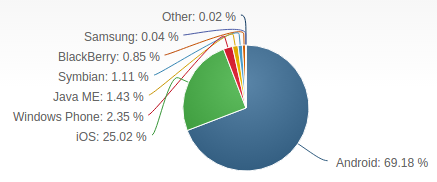
\includegraphics[width=\textwidth]{./images/netmarketshare201609-mobileOS}
                \caption[font=tiny]{\href{https://www.netmarketshare.com/operating-system-market-share.aspx?qprid=8&qpcustomd=1}{NetmarketShare (September 2016)}}
        	\end{figure}
	\end{frame}

	\begin{frame}
	\frametitle{Introducing Android}
	\framesubtitle{Java code everywhere (Android \& Beyond)}
	\begin{columns}
	\column{0.5\textwidth}
		\begin{itemize}
			\item Study using data from the job site Indeed
			\item What languages do professionals use? Which ones are most in demand?
			\item Also see the \href{http://www.tiobe.com/tiobe-index/}{TIOBE Index}
			\item and the \href{http://spectrum.ieee.org/static/interactive-the-top-programming-languages-2016}{IEEE ranking (July 2016) (try all rankings)}
		\end{itemize}
	\column{0.5\textwidth}
	%More content goes here
	        \begin{figure}[h]
                \centering
                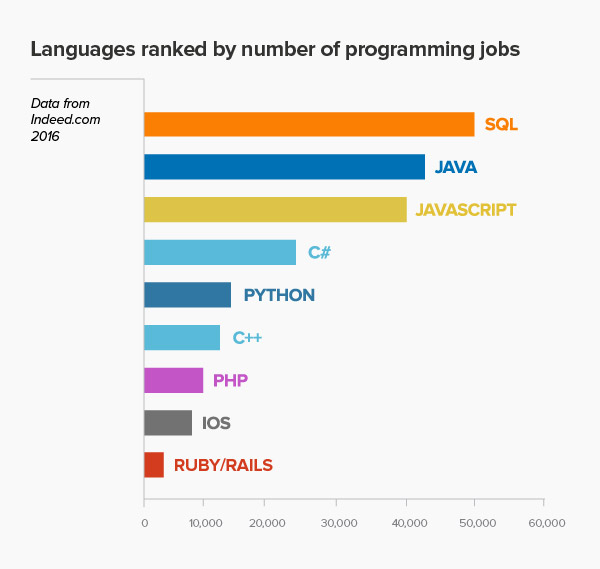
\includegraphics[width=\textwidth]{./images/Programming-Languages-for-2016_graph}
                \caption[font=tiny]{\href{http://www.codingdojo.com/blog/9-most-in-demand-programming-languages-of-2016/}{Coding Dojo (Jan 2016)}}
        	\end{figure}
	\end{columns}
	\end{frame}

	\begin{frame}
	\frametitle{Introducing Android}
	\framesubtitle{A moving target for developers}
	        \begin{figure}[h]
                \centering
                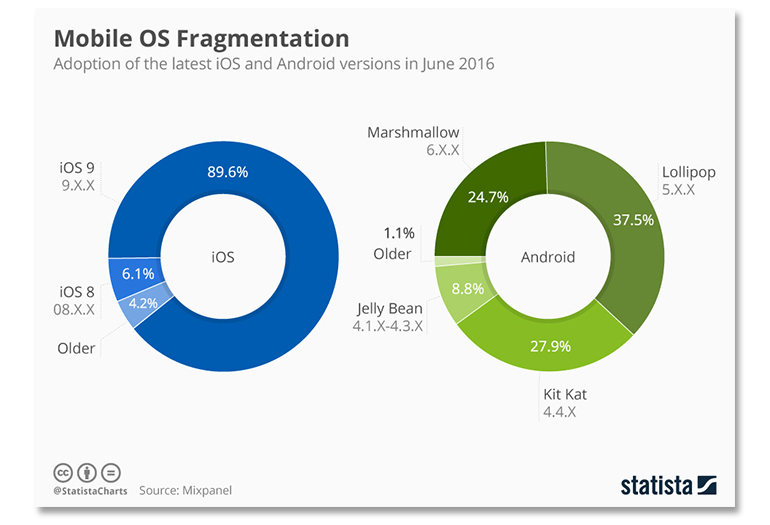
\includegraphics[width=0.8\textwidth]{./images/syme-ios-v-android}
        	\end{figure}
	\end{frame}

	
%%%%%%%%%%%%%% 2nd SECTION: Installing Android Studio %%%%%%%%%%%%%%%%%
\section[Section]{Setting Up your Dev Environment}
	\begin{frame}
	\frametitle{Computer Basics}
	\framesubtitle{Concepts to keep in mind}
	\begin{itemize}
		\item OS: operating system (Windows, Mac, Linux...)
		\item IDE: Integrated Development Environment (e.g. Android Studio, Eclipse)
		\item Console (to write) vs. IDE (to click): use the best tool for the job
		\item Server-side: your Android app might just be a client talking to a server
	\end{itemize}
	\end{frame}

	\begin{frame}
	\frametitle{Installing Android Studio on Linux}
	\framesubtitle{The way to go -e.g. on a Ubuntu-based distro}
	%More content goes here
	Install Oracle Java (the last step is optional):\\
	\texttt{\$ sudo add-apt-repository ppa:webupd8team/java\\
	\$ sudo apt-get update\\
	\$ sudo apt-get install oracle-java8-installer\\
	\$ sudo apt-get install oracle-java8-set-default\\
	}
	\vspace{1em}
	run  this to install Android Studio:\\
	\texttt{\$ sudo add-apt-repository ppa:paolorotolo/android-studio\\
	\$ sudo apt-get update\\
	\$ sudo apt-get install android-studio\\
	}
	\vspace{1em}
	Voilà!\\
	Executable should appear in the menus, or find it at \texttt{/opt/android-studio/bin/studio.sh}
	\end{frame}

	\begin{frame}
	\frametitle{Installing Android Studio on Linux}
	\framesubtitle{Follow the Wizard}
	        \begin{figure}[h]
                \centering
                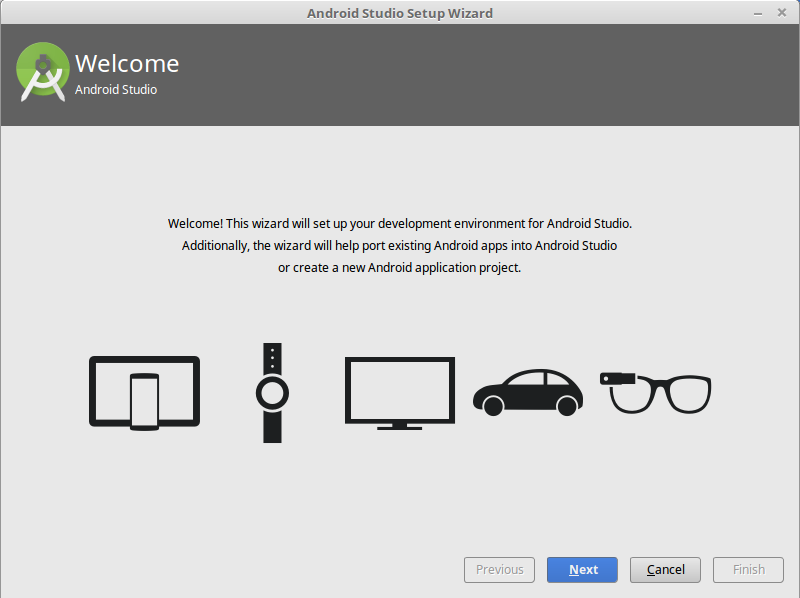
\includegraphics[width=0.8\textwidth]{./images/android-studio-wizard1}
        	\end{figure}
	\end{frame}
% See for KVM installation on Linux Mint (to run Android Emulator in accelerated performance mode): https://community.linuxmint.com/tutorial/view/1555

	\begin{frame}
	\frametitle{Installing Android Studio on Any Desktop}
	Follow instructions at \url{https://developer.android.com/studio/install.html}
	\end{frame}

	\begin{frame}
	\frametitle{Starting Development}
	        \begin{figure}[h]
                \centering
                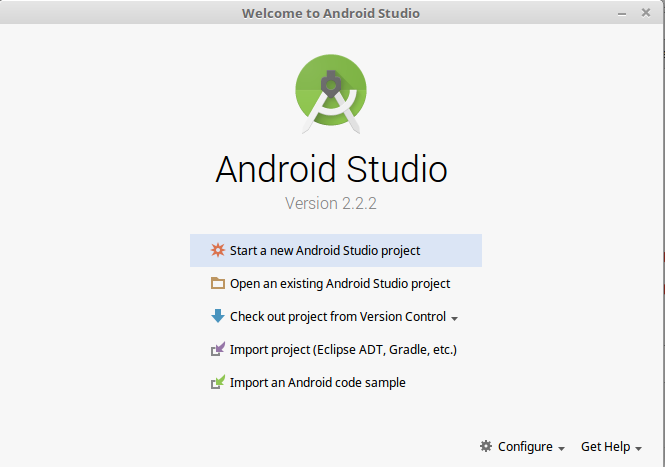
\includegraphics[width=0.8\textwidth]{./images/android-studio-startpage}
        	\end{figure}
	\end{frame}




%%%%%%%%%%%%%% 3rd SECTION: Learning the Language %%%%%%%%%%%%%%%%%
\section[Section]{Learning the Language}
	\begin{frame}
	\frametitle{How do you Learn a Language?}
	\framesubtitle{Building your dream apps on Android}
	% Babies learn talking, then learn reading => READ CODE
	%More content goes here
	\begin{itemize}
		\item Babies didn't learn at school!
		\item Read code, then read more code, then read more
		\item Write code, then write some more, then go and write more...
		\item Practice leads to perfection
	\end{itemize}
	\end{frame}

	\begin{frame}
	\frametitle{Resources to Learn Android}
	\framesubtitle{Excellent free books and videos out there}
	%More content goes here
	\begin{itemize}
		\item \url{https://developer.android.com/training/index.html}
		\item Google course on Udacity (60 hours): \url{https://www.udacity.com/course/developing-android-apps--ud853}
		\item Next steps is \href{https://www.udacity.com/course/android-developer-nanodegree-by-google--nd801?v=ad1}{Nanodegree} (not free: US\$250/month)
		\item \href{https://www.safaribooksonline.com}{Safari Books Online from O'Reilly (free with a Toronto Public Library card)}
		\item Don't forget to learn Java! See this great reference: \url{http://www.greenteapress.com/thinkapjava/thinkapjava.pdf}
	\end{itemize}
	\end{frame}


	\begin{frame}
	\frametitle{Final Words of Advice}
	\framesubtitle{To get really good at anything in life}
	%More content goes here
	\begin{itemize}
		\item Set high expectations for yourself
		\item Love what you do
		\item Never stop until you get there
	\end{itemize}
	\end{frame}

	\begin{frame}
	\frametitle{The End}
	\framesubtitle{}
	%More content goes here
	\centering
	Happy programming for Android!
	\end{frame}

\end{document}

